\section{Method}

We adapt the group lasso paradigm used to select independent dictionary elements in \citet{Koelle2022-ju, Koelle2024-no} to select pointwise isometries from a dictionary.
In particular, we first will define a ground truth objective computable via brute and greedy algorithms that is uniquely minimized by orthonormal matrices.
We then define the combination of normalization and multitask basis pursuit that approximates this ground truth loss function.
We finally give a brute post-processing method for ensuring that the solution is $D$ sparse.

\subsection{Ground truth}
\label{sec:ground_truth}

We'd like a ground truth objective to be minimized uniquely by orthonormal matrices, invariant under rotation, and depend on all changes in the matrix.
Deformation \citep{Kohli2021-lr} and nuclear norm \citep{Boyd2004-ql} use only a subset of the differential's information and are not uniquely minimized at unitarity, respectively.
We therefore introduce an alternative ground truth objective that satisfies the above desiderata and has convenient connections to Isometry Pursuit.

We define this objective as
\begin{align}
l_{c}: \mathbb R^{D \times P} &\to \mathbb R^{+} \\
X &\mapsto \sum_{d = 1}^D g(\sigma_d( X), c)
\end{align}
where $\sigma_d ( X)$ is the $d$-th singular value of $ X$ and
\begin{align}
g: \mathbb R^+ \times \mathbb R^+ &\to \mathbb R^+ \\
t,c &\mapsto \frac{e^{t^c} + e^{t^{-c}}}{2e}.
\end{align}
Using Proposition \ref{prop:orthonormal_spectrum}, we can check that $g$ is uniquely maximized by orthonormal matrices.
Moreover, $g( X^{-1}) = g( X)$ and $g$ is convex.
Figure \ref{fig:losses} gives a graph of $l_c$ when $D=1$ and compares it with that produced by basis pursuit after normalization as in Section \ref{sec:normalization}.
% NOTE (Sam): Do we need proofs of maximized by orthonormal matrices and convex?
% Can we prove this is a norm?

Our ground truth program is therefore 
\begin{align}
\label{prog:ground_truth}
\widehat { S}_{GT}  &= \arg \min_{ S \in \binom{[P]}{d}} l_c ( X_{. S}).
\end{align}
Regardless of the convexity of $l_c$, brute combinatorial search over $[P]$ is inherently non-convex.

\subsection{Normalization}
\label{sec:normalization}

Since basis pursuit methods tend to select longer vectors, selection of orthonormal submatrices requires normalization such that both long and short candidate basis vectors are penalized in the subsequent regression.
We introduce the following definition.

\begin{definition}[Symmetric normalization]
A function $q: \mathbb R^D \to \mathbb R^+ $ is a symmetric normalization if 
\begin{align}
\arg \max_{v \in \mathbb R^D} \ q (v) &=\{ v : \|v\|_2 = 1 \} \\
q(v) &= q(\frac{v}{\|v\|_2^2}) \\
q(v_1) &= q(v_2) \; \forall v_1, v_2 \in \mathbb R^D : \|v_1\|_2 = \|v_2\|_2.
\end{align} \label{def:symmetric_normalization}
\end{definition}

We use such functions to normalize vector length in such a way that vectors of length $1$ prior to normalization have longest length after normalization, vectors in general are shrunk proportionately to their deviation from $1$. 
That is, we normalize vectors by 
\begin{align}
n: \mathbb R^D  &\to \mathbb R^D \\
v &\mapsto {q(v) }v
\end{align}
and matrices by
\begin{align}
w: \mathbb R^{D \times P}  &\to \mathbb R^D \\
 X_{.p} &\mapsto n( X_{.p}) \; \forall p \in [P].
\end{align}

In particular, given $c > 0$, we choose $q$ as follows.
\begin{align}
\label{eq:normalization}
q_c: \mathbb R^D  &\to \mathbb R^+ \\
v  &\mapsto \frac{e^{\|v\|_2^c} + e^{\|v\|_2^{-c}}}{2e}.
\end{align}

Besides satisfying the conditions in Definition \ref{def:symmetric_normalization}, this normalization has some additional nice properties.
First, $q$ is convex.
Second, it grows asymptotically log-linearly.
Third, while $\exp(-|\log t|) = \exp(-\max (t, 1/t))$ is a seemingly natural choice for normalization, it is non smooth, and the LogSumExp replacement of $\max (t, 1/t)$ with $ \log (\exp (t ) + \exp(1/t))$ simplifies to \ref{eq:normalization} upon exponentiation \citep{Boyd2004-ql}.
Finally, the parameter $c$ grants control over the width of the basin, which is important in avoiding numerical issues arising close to $0$ and $\infty$.

\begin{figure}
\centering
\subcaptionbox{Ground truth loss scaling function $g$ as a function of $t$. \label{cat}}
{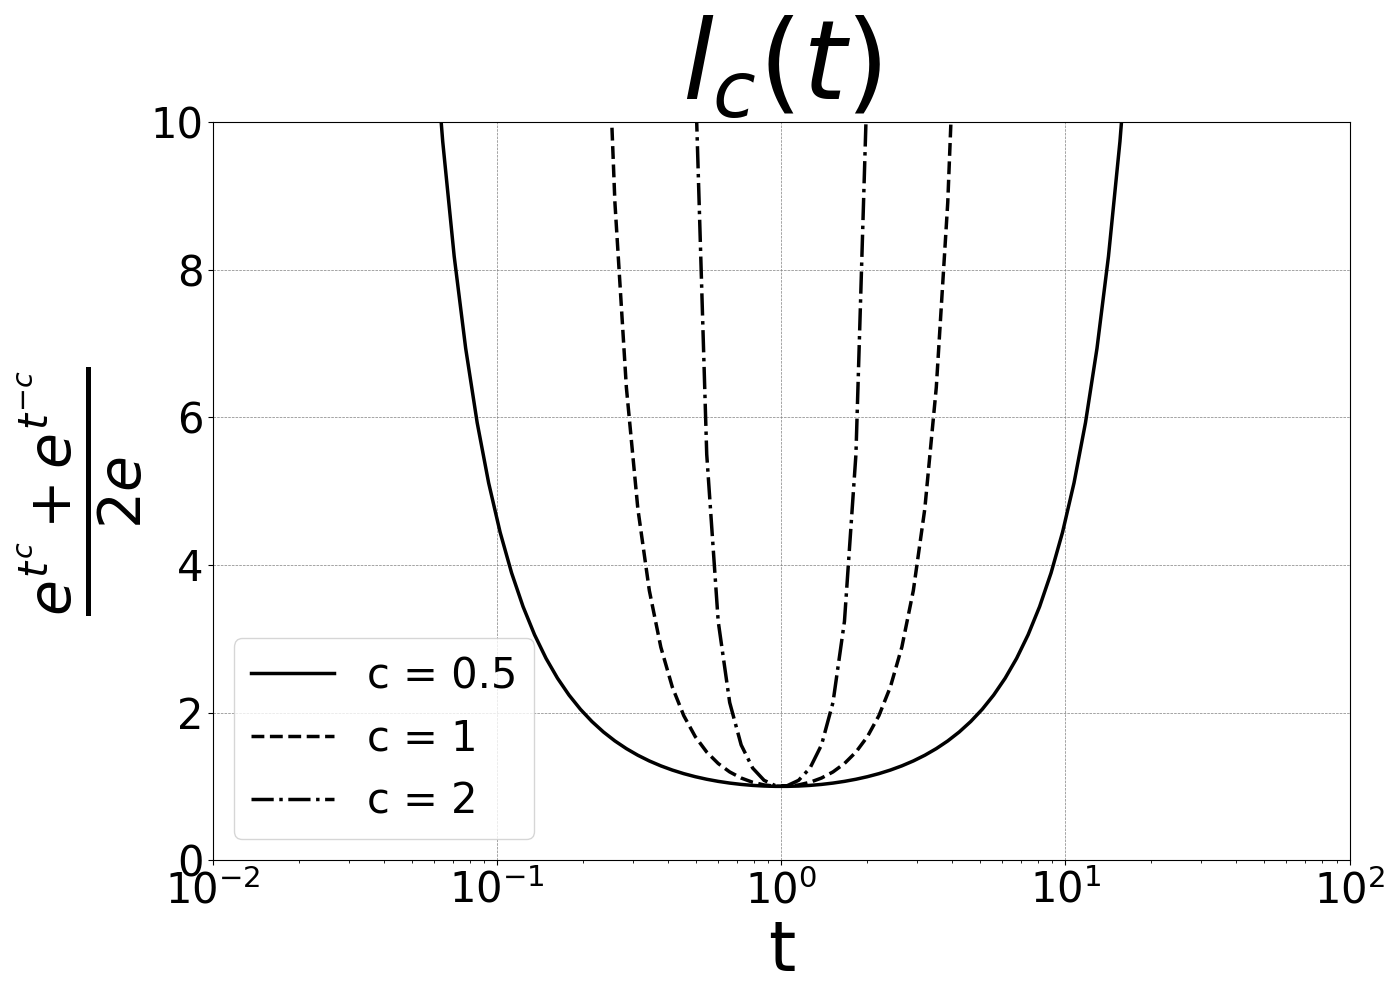
\includegraphics[width = .32\textwidth]{../figures/Figure_1a_bw.png}}
\label{fig:gt_loss}
\subcaptionbox{Length as a function of $t$ \label{elephant}}
{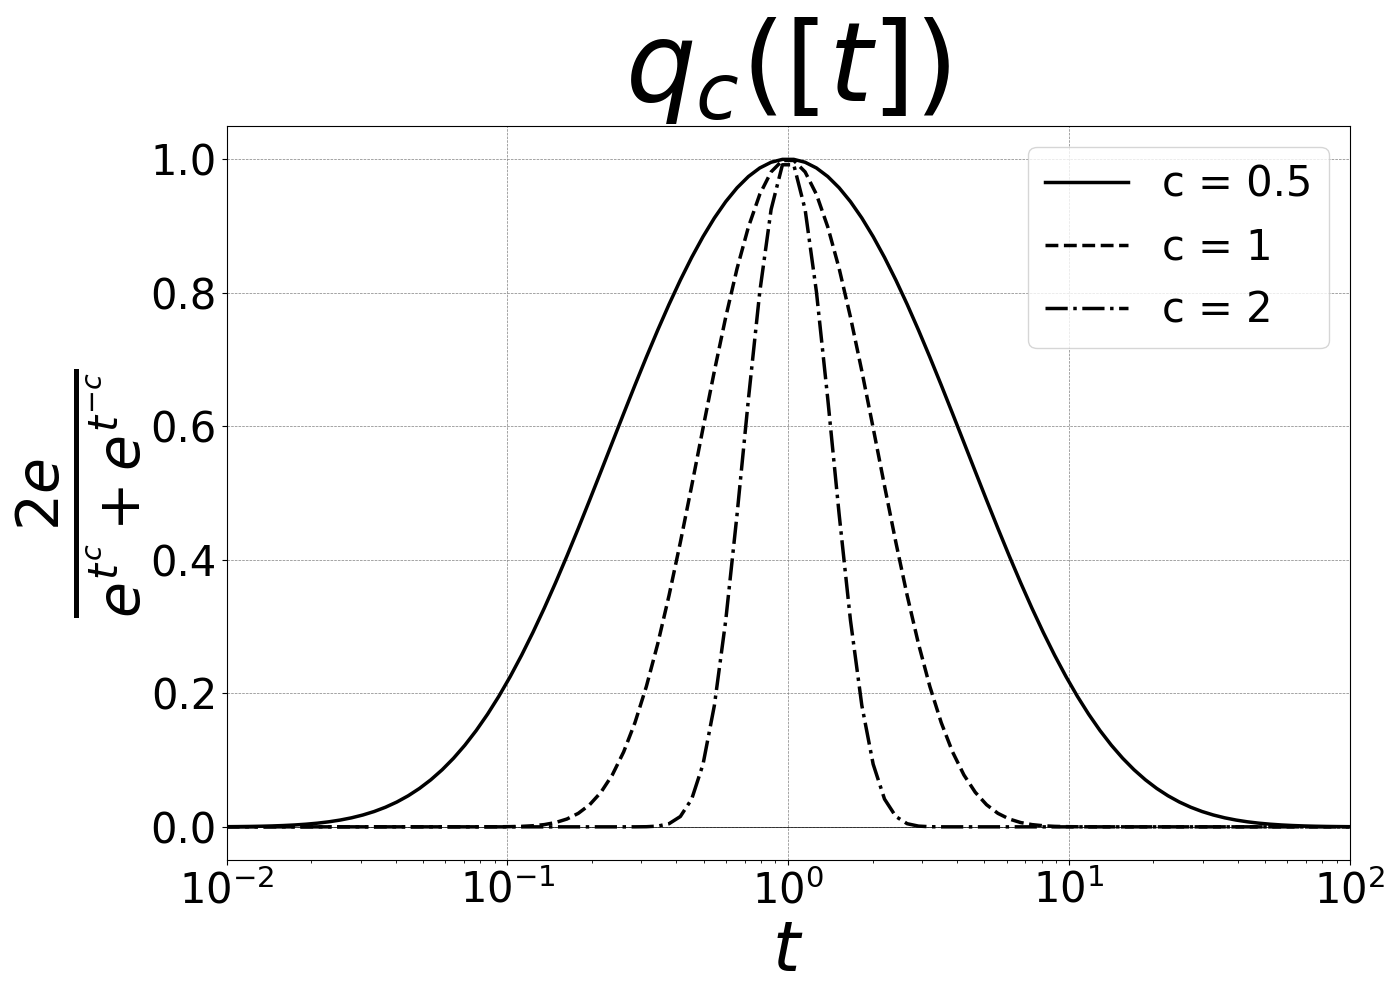
\includegraphics[width = .32\textwidth]{../figures/Figure_1b_bw.png}}
\subcaptionbox{Basis pursuit loss as a function of $t$ \label{snootfellow}}
{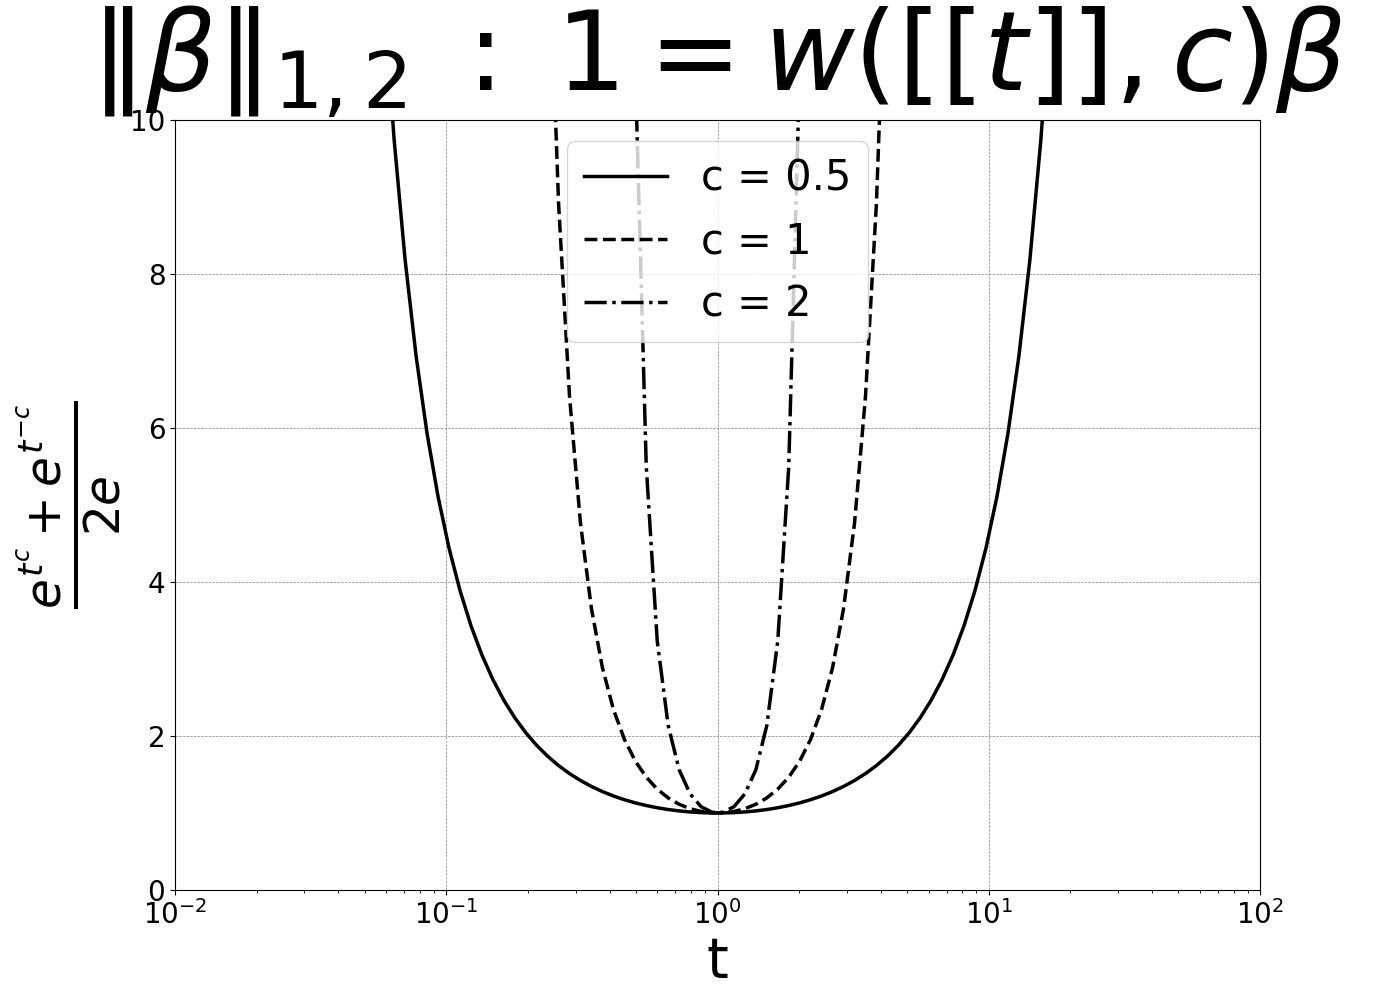
\includegraphics[width = .32\textwidth]{../figures/Figure_1c_bw.png}}
\caption{Plots of ground truth loss, normalized length, and basis pursuit loss for different values of $c$ in the one-dimensional case $D = 1$.
The two losses are equivalent in the one-dimensional case.}
\label{fig:losses}
\end{figure}

\subsection{Isometry pursuit}

Isometry pursuit is the application of multitask basis pursuit to the normalized design matrix $w(X, c)$ to identify submatrices of $ X$ that are as orthonormal as possible.
Define the multitask basis pursuit penalty 
\begin{align}
\label{eq:bp}
\| \cdot \|_{1,2}: \mathbb R^{P \times D} &\to \mathbb R^+ \\ 
\beta &\mapsto  \sum_{p=1}^P  \|\beta_{p.}\|_2.
\end{align}
Given a matrix $Y \in \mathbb R^{D \times E}$, the multitask basis pursuit solution is
\begin{align}
\label{prog:multitask_basis_pursuit}
\widehat \beta_{MBP} (X, Y)  := \arg \min_{\beta \in \mathbb R^{P \times E}} \| \beta \|_{1,2} \; : \;Y =  X \beta.
\end{align}
Isometry pursuit is then given by
\begin{align}
\label{prog:isometry_pursuit}
\widehat \beta_c ( X) := \widehat \beta_{MBP} ( w(X,c), I_D )
\end{align}
where $I_D$ is the $D$ dimensional identity matrix and recovered functions are the indices of the dictionary elements with non-zero coefficients.
That is, they are given by $S(\beta)$ where
\begin{align}
S: \mathbb{R}^{p \times d} &\to \binom{[P]}{d} \\
\beta &\mapsto \left\{ p \in [P] :  \|\beta_{p.}\| > 0 \right\}.
\end{align}
\begin{algorithm}[H]
\caption{\isometrypursuit(Matrix ${X} \in \mathbb{R}^{D \times P}$, scaling constant $c$)}
\begin{algorithmic}[1]
\STATE {Normalize} $X_c = w({X},c)$
\STATE {Optimize} $\widehat \beta = \widehat \beta_{MBP} (X_c, I_D)$
\STATE {\bf Output} $\widehat{S} = S (\widehat \beta)$
\end{algorithmic}
\end{algorithm}

\subsection{Theory}

The intuition behind our application of multitask basis pursuit in our setting is that submatrices consisting of vectors which are closer to 1 in length and more orthogonal will have smaller loss.
A key initial theoretical assertion is that  \isometrypursuit~ is invariant to choice of basis for $ X$.
\begin{proposition}
\label{prop:basis_pursuit_selection_invariance}
Let $U \in \mathbb R^{D \times D}$ be orthonormal.
Then $S(\widehat \beta  (U  X)) = S(\widehat \beta ( X))$.
\end{proposition}
A proof is given in Section \ref{proof:basis_pursuit_program_invariance}.
This has as an immediate corollary that we may replace $I_D$ in the constraint by any orthonormal $D \times D$ matrix.

We also claim that the conditions of the consequent of Proposition \ref{prop:orthonormal_basis} are satisfied by minimizers of the multitask basis pursuit objective applied to suitably normalized matrices in the special case where both such a submatrix exists and $| S| = D$.
\begin{proposition}
Let $w_c$ be a normalization satisfying the conditions in Definition \ref{def:symmetric_normalization}.
Then $\arg \min_{X_{.S} \in \mathbb R^{D \times D}} \widehat \beta^{D}_c ( X) $ is orthonormal.
Moreover when $X$ is orthonormal, $(\min_{\beta \in \mathbb R^{P \times D}} \| \beta \|_{1,2} \; : \; I_D = w ({  X}, c) \beta) = D$.
\label{prop:unitary_selection}
\end{proposition}
While this Proposition falls short of showing that an orthonormal submatrix will be selected should one be present, it provides intuition justifying the preferential efficacy of \isometrypursuit~ on real data.
A proof is given in Section \ref{sec:local_isometry_proof}.

\subsection{Two-stage isometry pursuit}

Since cannot in general ensure either that $|\widehat {  S|} = D$ or that a orthonormal submatrix $X_{.S}$ exists, we first use the convex problem to prune and then apply brute search upon the substantially reduced feature set.

\begin{algorithm}[H]
\caption{\tsip(Matrix ${X} \in \mathbb{R}^{D \times P}$, scaling constant $c$)}
\begin{algorithmic}[1]
\STATE $\widehat{S_1} = \text{\isometrypursuit}( X, c)$
\STATE $\widehat{S} = \text {\brute}({X}_{.\widehat{S_1}}, l_c)$
\STATE {\bf Output} $\widehat{S}$
\end{algorithmic}
\end{algorithm}

Similar two-stage approaches are standard in the Lasso literature \cite{Hesterberg2008-iy}.